\subsection{Chinese anti-leverage}

Figure~\ref{fig:rhos} summarises the results by plotting the posterior densities of $\rho$ obtained from all the model fits.
Even though not all companies behave the same way, there is a consistent picture in general about the differences between the two countries.
The chart shows that, based on the chosen sample, $\rho$ is really estimated to be larger in China than in Germany, except for the periods containing the crisis, when it was similar.

The claims about China behaving differently are underpinned by Figure~\ref{fig:negative-rhos}, which shows the number of companies with a significant leverage or anti-leverage effect.
We define significance at the 5\% level in this master thesis, i.e.\ significant leverage means that the 95\% quantile of $\rho$'s posterior is negative, while significant anti-leverage means that the 5\% quantile of $\rho$'s posterior is positive.
Interestingly, Germany had the least number of companies with significant leverage effect in the period that just preceded the crisis, which was followed by a steep increase into the crisis.
Apart from the periods containing the boom phase of the Subprime Crisis or touching the European Debt Crisis, the figure for Germany is quite stable around 6 to 7.
None of the German stocks had a significantly positive $\rho$.

The picture is much less consistent about China.
Ignoring periods with only one significant value, the leverage effect is only present under the crisis of 2007, with some delay compared to Germany, and only in 3 stocks at most.
Similarly, anti-leverage is hardly observed, only before the crisis.
Still, the companies show some consistency, since there is no period with both leverage and anti-leverage effect being present.

\comment{
Note that the exact distribution or point estimates of $\rho$ are not of high interest.
On the one hand, it is not the correlation of returns with variance changes but with log variance changes, which makes it more difficult to interpret.
On the other hand, comparison with correlation values obtained from other models in the literature is also not trivial, so across models only the sign and highly extreme values are interesting.
}

\subsection{Time-varying leverage}

Figures~\ref{fig:rhos} and~\ref{fig:negative-rhos} suggest that leverage is not constant, even its sign varies.
The charts show that correlation shifts to the negative direction throughout the crisis, which is consistent with recent literature~\citep{Christensen2015}.
It seems to hold especially for the Chinese stocks since the German companies are more stably on the negative side throughout the whole time.

Figure~\ref{fig:company-rhos} shows how the posterior of $\rho$ changes for each company with the rolling window of periods.
The German stocks are on the bottom half of the chart, they have a significant leverage effect in general since the crisis.
They show a quite consistent picture, the 95\% quantile is negative for the vast majority of estimates.
BMW and SAP show a steadily strengthening leverage effect, while it stagnates or weakens for the others.
If we accept that the leverage effect is stronger in crises~\citep{Christensen2015}, then the increasing $\rho$ in 8 out of the 10 German companies signals the end of the impact of recent crises.

The posterior $\rho$ developed far more hectically for the Chinese companies.
However, they all had the negative extremum of the posteriors around the first half of 2008, at the strongest impact of the crisis.
However, the overall picture is unstable throughout the whole examined time, which questions the reliability of the results from the perspective of~\citet{Christensen2015}.
There might be far more and substantially different factors in play that affect Chinese stocks' leverage effect.

\subsection{Volatility estimations}

The posterior of $\phi$ and of the log variance are presented in Figure~\ref{fig:persistence} on a chosen subset of periods and companies that represent the whole dataset.
The prior of $\phi$ is taken to be informative, it reflects the empirical fact of highly autocorrelating volatility.
The posterior of $\phi$ mainly depends on its prior and the estimate for $\bm h$.
Hence, if the posterior is significantly different from the prior, that means that there is valuable information in $\bm h$ about $\phi$.

An immediately noticeable phenomenon in Figure~\ref{fig:persistence} is that the posterior of $\phi$ varies more for the German firms.
More precisely, throughout the crisis and in its short aftermath, the volatility of the German stocks was substantially more persistent than in the other periods.
At the same time, changes in the persistence of the Chinese companies can not be explained by the crisis periods, and the estimates are more stable and closer to the prior, except for the highly persistent 2010-2012 period of 600016 CH Equity.
One can also spot the differences on the log variance timeline: the time series are close to a constant value plus noise in China, containing little information about persistence.
In Germany, on the other hand, clusters of increasing and decreasing trends can be observed around the crisis.

\begin{figure}[p]
	\vspace*{-3.2cm}
	\centering
	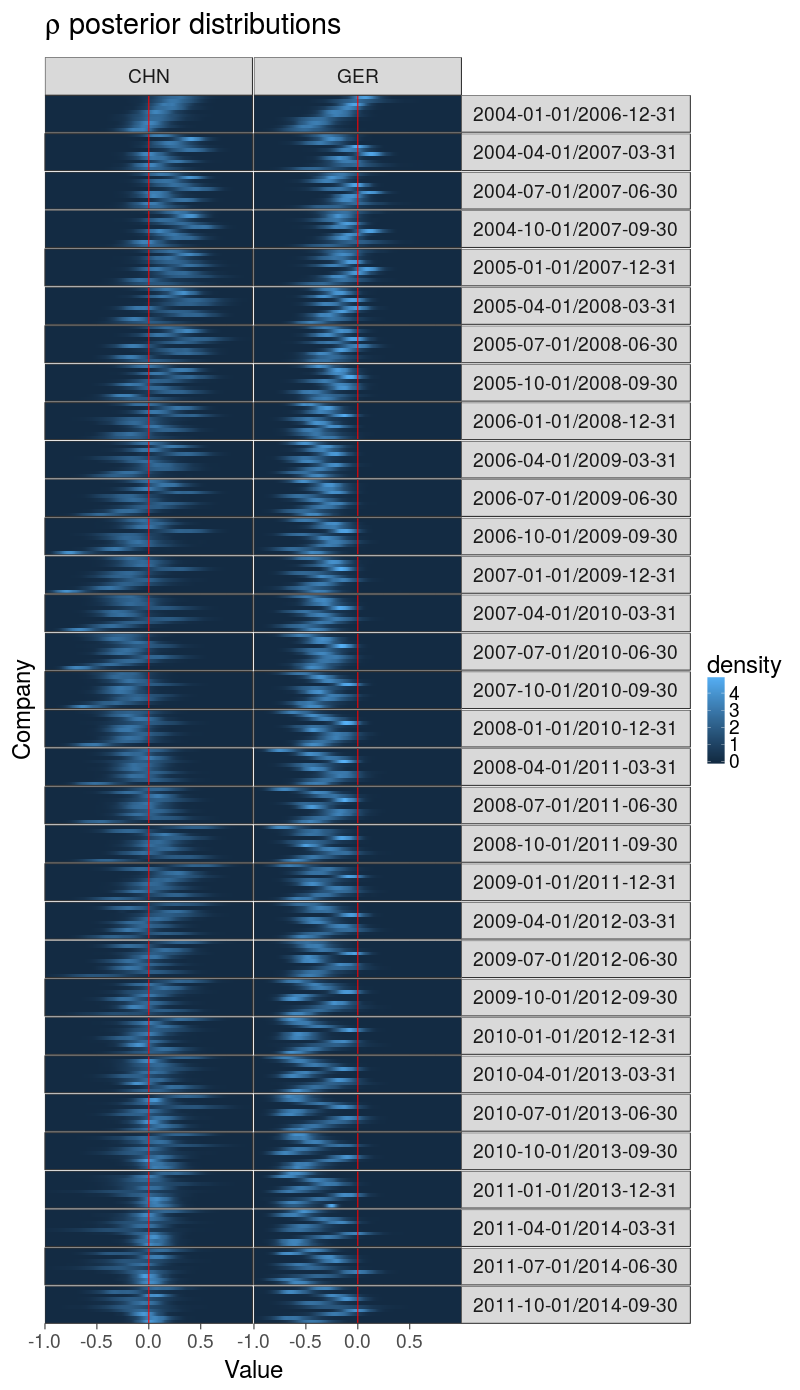
\includegraphics[width=\linewidth]{../calculations/rhos.pdf}
	\caption[Visually summarising the results]{Visually summarising the results. Each blue box corresponds to a country and a period and contains 10 rows. One row corresponds to one stock. Each row is a heatmap of $\rho$'s posterior density estimated for that company and period. The red line is constant 0. The stocks' rows are ordered according to their posterior mean in the first period.}
	\label{fig:rhos}
\end{figure}

\begin{figure}[p]
	\vspace*{-3.2cm}
	\centering
	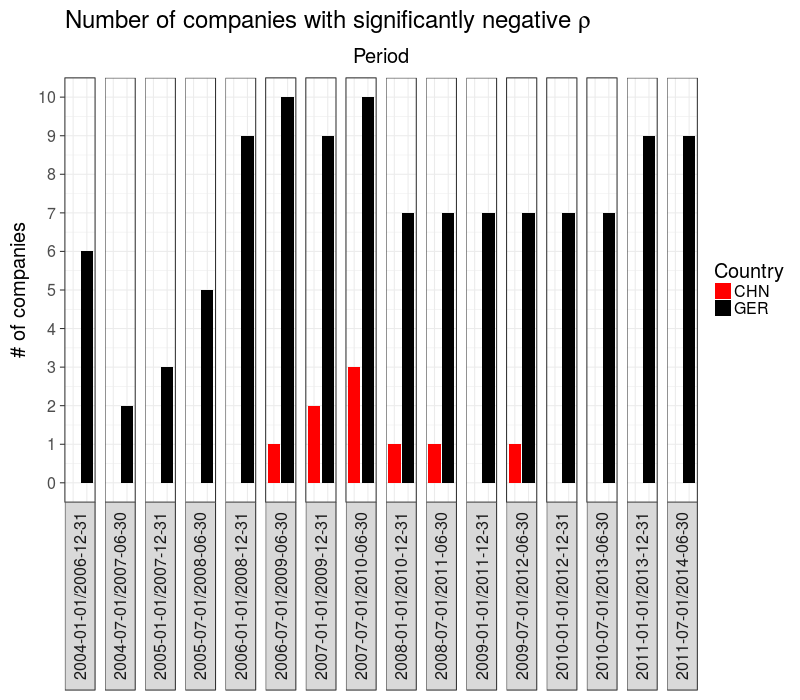
\includegraphics[width=\linewidth]{../calculations/negative-rhos.pdf}
	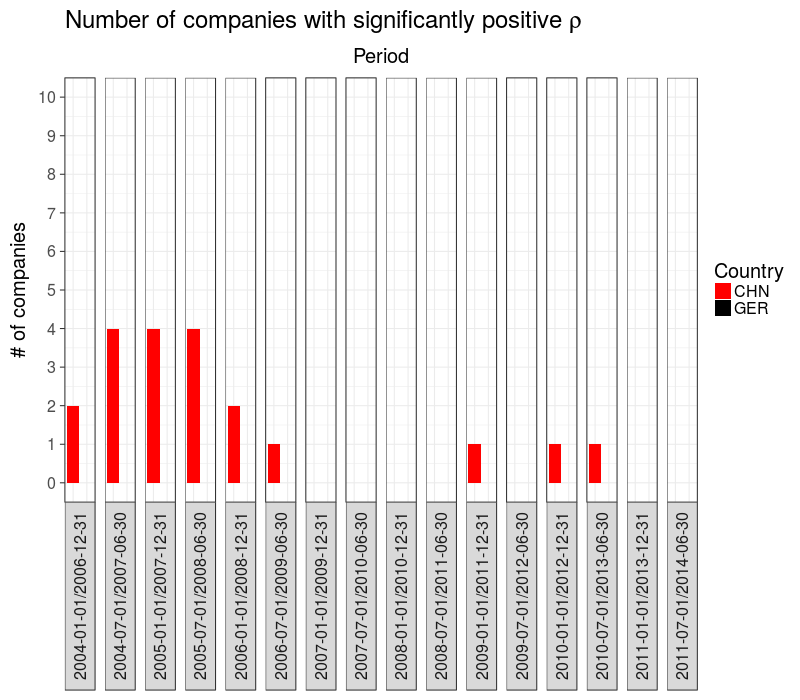
\includegraphics[width=\linewidth]{../calculations/positive-rhos.pdf}
	\caption[Significant leverage effect]{Top: number of companies with significant leverage effect per country and period, on a 5\% level. Bottom: number of companies with significant anti-leverage effect per country and period, on a 5\% level. Both: Only every second period is shown for readability.}
	\label{fig:negative-rhos}
\end{figure}

\begin{figure}[p]
	\vspace*{-3.2cm}
	\centering
	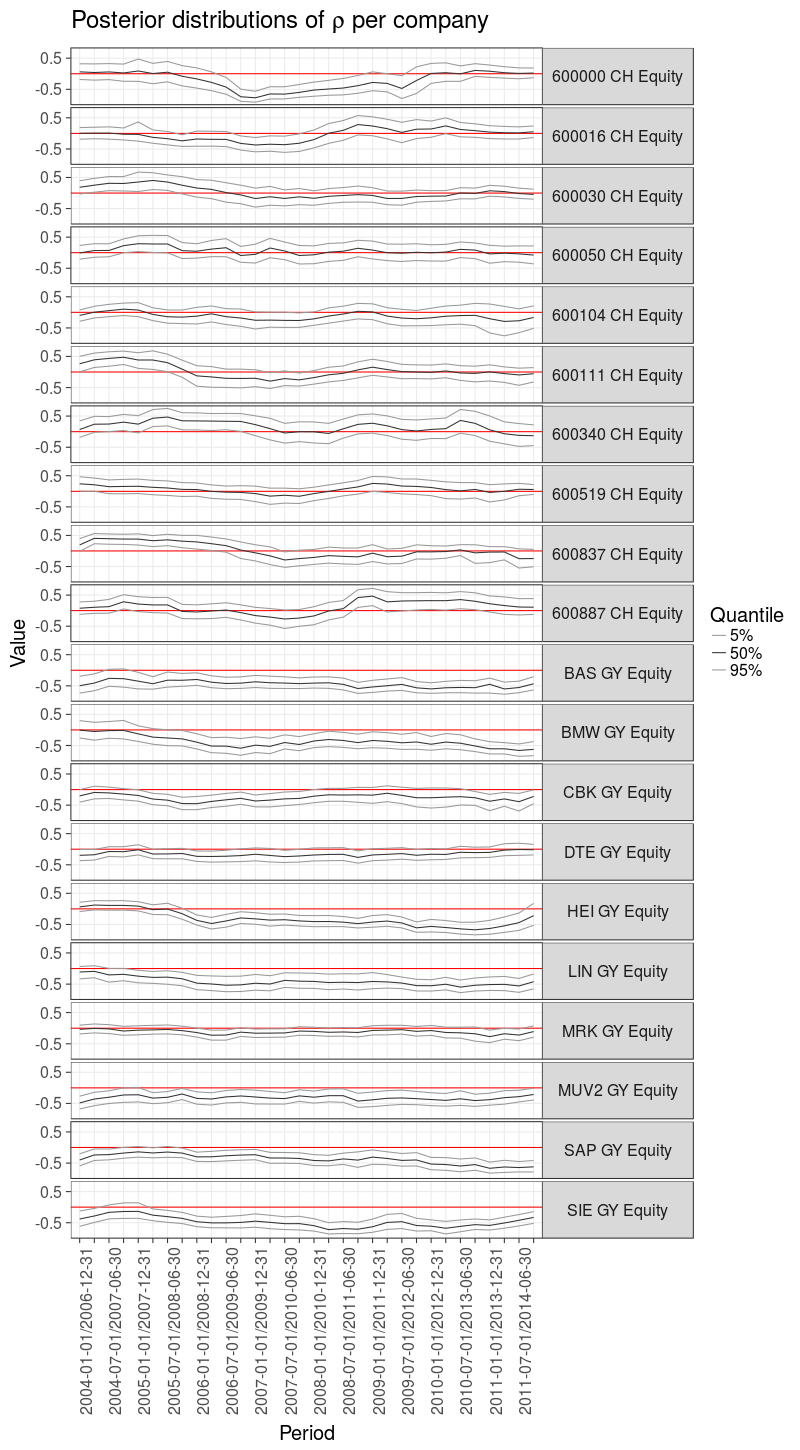
\includegraphics[width=\linewidth]{../calculations/rho-timeline.pdf}
	\caption[Timeline of posterior $\rho$]{Posterior distributions of $\rho$ in time. The prior distribution is the uniform distribution on $[-1,1]$ in all cases.}
	\label{fig:company-rhos}
\end{figure}

\begin{figure}[p]
	\vspace*{-3.2cm}
	\centering
	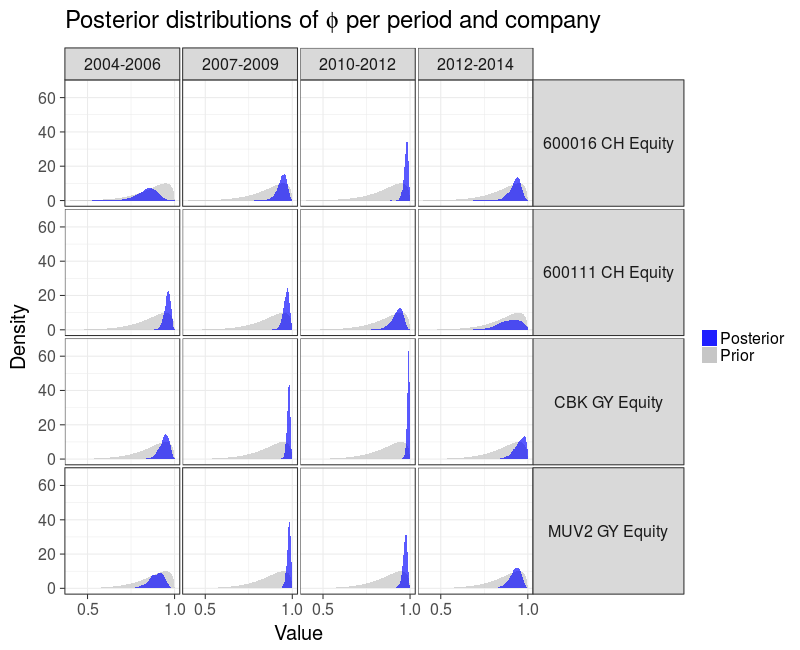
\includegraphics[width=\linewidth]{../calculations/phi-timeline.pdf}
	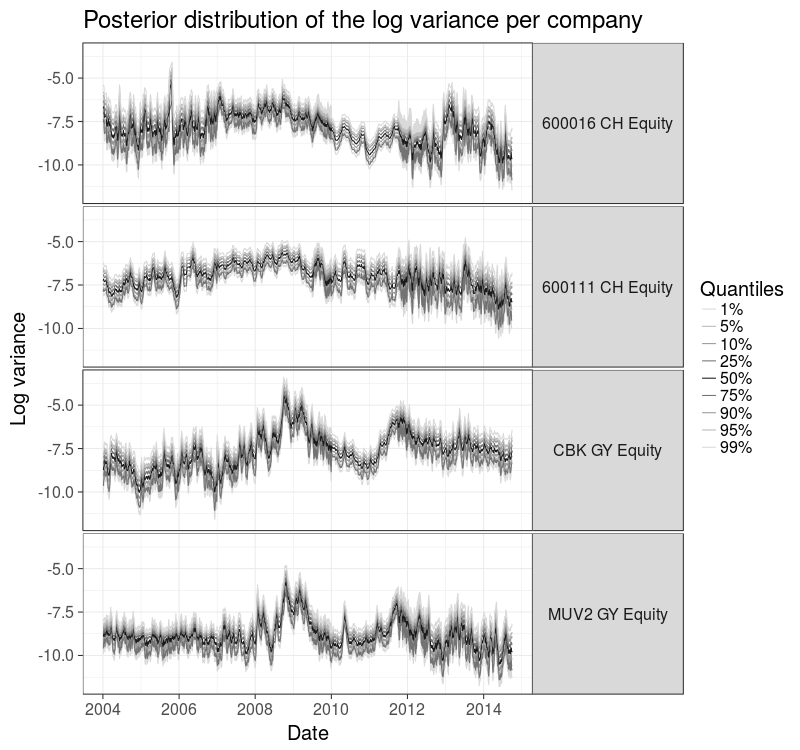
\includegraphics[width=\linewidth]{../calculations/volatility.pdf}
	\caption[Timeline of persistence and volatility]{Top: posterior persistence of the log variance for a subset of companies and periods. Bottom: posterior log variance for a subset of the companies. The time series are glued together from the independent volatility estimations from several periods.}
	\label{fig:persistence}
\end{figure}
